\section{I modelli del traffico}
\begin{center}
	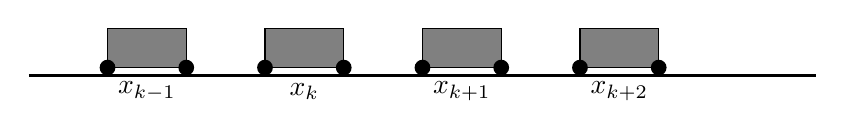
\begin{tikzpicture}
		\draw[draw=black,thick] (-5,-0.1) -- (5,-0.1);
		\filldraw[fill=gray,draw=black] (-4,0) rectangle (-3,0.5);
		\node at (-3.5,-0.3) {$x_{k-1}$};
		\fill[fill=black] (-4,0) circle (0.1cm);
		\fill[fill=black] (-3,0) circle (0.1cm);
		
		\filldraw[fill=gray,draw=black] (-2,0) rectangle (-1,0.5);
		\node at (-1.5,-0.3) {$x_{k}$};
		\fill[fill=black] (-2,0) circle (0.1cm);
		\fill[fill=black] (-1,0) circle (0.1cm);
		
		\filldraw[fill=gray,draw=black] (0,0) rectangle (1,0.5);
		\node at (0.5,-0.3) {$x_{k+1}$};
		\fill[fill=black] (0,0) circle (0.1cm);
		\fill[fill=black] (1,0) circle (0.1cm);
		
		\filldraw[fill=gray,draw=black] (2,0) rectangle (3,0.5);
        \node at (2.5,-0.3) {$x_{k+2}$};
        \fill[fill=black] (2,0) circle (0.1cm);
        \fill[fill=black] (3,0) circle (0.1cm);	
    
	\end{tikzpicture}
\end{center}

Modellizziamo il traffico su una strada ad una sola corsia considerando $N$ macchine su una strada lunga $L$; per ogni macchina conosciamo la posizione al tempo $t$ che è data dalla funzione $x_k(t)$, chiaramente $\dot{x_k(t)}$ rappresenta la velocità della k-esima macchina.
\paragraph{Car following model}
Per descrivere questo sistema possiamo usare vari approcci: per esempio potremmo supporre che la velocità di ogni macchina sia regolata dalla velocità della successiva e vari in maniera tale da uguagliare le due velocità.
 Inoltre dobbiamo supporre che ci sia un ritardo $\tau$ nella risposta dell'automobilista che quindi fa si che la velocità si regoli sulla velocità percepita ad un tempo $t-\tau$, così facendo otteniamo un modello di questo tipo:

\begin{equation}
	\ddot{x}_k(t)=\gamma(\dot{x}_{k+1}(t-\tau)-\dot{x}_{k}(t-\tau))
			 \label{diifeqcarfollowing}
\end{equation}
\paragraph{Optimal velocity model}Potremmo però supporre anche un secondo tipo di modello basato sull'assunzione che ogni macchina cerchi di regolare la sua velocità cercando di raggiungere una velocità ottimale dipendete dalla distanza con il veicolo successivo ($v_{opt}(\Delta x_k)$) che ottimizzi sia la rapidità con cui si effettua un tragitto sia la probabilità di fare incidenti. \\ Dobbiamo però capire che tipo di forma analitica ha questa $v_{opt}(\Delta x_k)$. 

\begin{multicols}{2}
	 Nel caso più semplice potremmo assumere che questa tenda a zero per una certa distanza minima $d_0$, in maniera tale da evitare incidenti, e allo stesso tempo tenda ad una velocità limite $v_\infty$, che potrebbe essere il limite di velocità imposto dal codice della strada, per distanze molto grandi. Una delle curve di cui abbiamo già parlato e che presenta un comportamento simile è proprio la funzione logistica:
	 \begin{equation}
	 	v_{opt}(\Delta x)= v_\infty(\tanh(a\Delta x-b)+\tanh(b))
	 	\label{optimalvelocity}
	 \end{equation}
	
	\begin{tikzpicture}
	\draw[->](0,0) -- (0,5) node[right] {$v_{opt}$};
	\draw[->](0,0) -- (5,0) node[right] {$\Delta x$};
	\draw[draw=blue] (1,0) .. controls (3,0.1) and (3.5,3.9) .. (5,3.9);
	\draw[thick] (1,-0.2)--(1,0.2) node[above] {$d_0$   };
	\draw[thick] (0.2,4)--(-0.2,4) node[left]{$v_\infty$};
	\draw[dotted, draw=gray](0,4)--(5,4);
	\end{tikzpicture}
	
\end{multicols}
La (\ref{optimalvelocity}) potrebbe non essere facilmente riconosciuta come funzione logistica ma è sufficiente esprimere le tangenti iperboliche in forma esponenziale per rendersi conto che è proprio una soluzione dell'equazione logistica di cui abbiamo già parlato. Così facendo possiamo scrivere un'equazione differenziale con ritardo, che si scopre avere una soluzione analitica. ,  ottenendo
\begin{equation}
	\dot{x}_k(t)=v_{opt}(\Delta x_k(t-\tau))
	\label{ovmdiffeq}
\end{equation} 
Per semplicità di calcolo applichiamo una traslazione ai tempi così che $t\rightarrow (t+\tau)$ e $(t-\tau)\rightarrow t$ e sviluppiamo in serie di Taylor per $\tau$ piccolo il termine $\dot{x}_k(t+\tau)\backsimeq \dot{x}_k(t)+\tau \ddot{x}_k(t)$, per cui otteniamo una nuova equazione valida solo per tempi di risposta brevi, che converte i termini di ritardo in un termine dissipativo che rende il sistema stabile quando la velocità di ogni macchina è quella ottimale.
\begin{equation}
	\ddot{x}_k(t)=-\frac{1}{\tau}(\dot{x}_k-v_{opt}(\Delta x_k(t))
	\label{eqddissipazione}
\end{equation}

Un secondo modo per studiare la (\ref{ovmdiffeq}) può essere quello di esplicitare tutto in funzione delle distanze tra le auto, così facendo abbiamo che:
\begin{equation}
	\begin{gathered}
		\Delta x_k=x_{k+1}-x_k \qquad \Rightarrow \qquad \dot{\Delta x}_k=\dot{x}_{k+1}-\dot{x}_{k}\\
		\dot{\Delta x}_k(t)=v_{opt}(\Delta x_{k+1}(t-\tau))-v_{opt}(\Delta x_{k}(t-\tau))
		\label{ovmdiffeqdist}
	\end{gathered}
\end{equation}
Quest'ultima forma mette in evidenza che le condizioni di equilibrio del sistema si raggiungono quando ogni macchina viaggia alla stessa velocità, ossia quella ottimale; dipendendo questa dalle distanze però è immediato osservare che perchè vi sia equilibrio allora è necessario che le macchine siano tutte equidistanziate.
\subsection{Flusso di traffico}

Vogliamo quindi sfruttare quanto abbiamo compreso per determinare se esiste una condizione in cui il traffico inizia a congestionarsi e quali sono le condizioni che evitano il congestionamento. Per cominciare allora definiamo due grandezze:
\begin{itemize}
	\item \textbf{Densità di traffico}: $\rho = \frac{N}{L}$, ossia il numero di macchine per unità di lunghezza della strada ($l=$ lunghezza strada e $N=\#$ macchine in strada).
	\item \textbf{Flusso di traffico}: $\Phi=\rho v_{opt}$, ovvero quanti veicoli fluiscono nell'unità di tempo nella strada.
\end{itemize}
La seconda definizione può apparire un po' controintuitiva ma in realtà se assumiamo che le auto si muovano alla velocità ottimale allora considerando il tempo di percorrenza della strada di una macchina $\Delta t$ è chiaro che $\Phi=\rho \frac{L}{\Delta t}=\rho v_{opt}$. Inoltre l'assunzione che tutte le macchine vadano alla velocità ottimale implica direttamente l'equilibrio del sistema poichè $\dot{\Delta x_k}=0$ e come abbiamo già osservato in questa condizione necessariamente tutti i veicoli devono essere equidistanti e quindi con distanza $\Delta x=\frac{L}{N}=\rho^{-1}$.
\begin{multicols}{2}
	\begin{tikzpicture}
		\draw[->](0,0) -- (0,3) node[right] {$\Phi$};
		\draw[->](0,0) -- (5,0) node[right] {$\rho$};
		\draw[draw=blue] (0,0) .. controls (2.5,4) and (2.7,1) .. (5,0.3);

	\end{tikzpicture}

Abbiamo quindi che il flusso dipenderà solamente dalla densità di macchine, se sono valide le condizioni assunte sopra, e quindi otteniamo chiaramente un punto di massimo di flusso oltre al quale la distanza di equilibrio tra le macchine diventa troppo piccola e le auto devono diminuire eccessivamente la loro velocità riducendo anche il flusso che può immettersi generando congestionamento.


\end{multicols}
Potremmo domandarci se questo punto di massimo è un equilibrio stabile o instabile: chiaramente è instabile poichè qualsiasi perturbazione di $\rho$ può generare una diminuzione di flusso, per cui non è conveniente attendersi che le strade debbano essere saturate di veicoli fino a questo livello. Ma allora qual'è la densità ottimale per una strada?\\

Per cominciare definiamo $u(t)=v_{opt}(\Delta x(t))$ per cui abbiamo subito $\dot{u}(t)=v'_{opt}(\Delta x)\dot{\Delta x}$ e applichiamo questo cambio di variabili alla (\ref{eqddissipazione}) ottenendo:
\begin{equation}
	\begin{cases}
		\dot{u_k}(t)=v'_{opt}(\Delta x_k)\dot{\Delta x_k}\\
		\ddot{\Delta x_k}=-\frac{1}{\tau}(\dot{\Delta x_k}-(u_{k+1}(t)-u_k(t)))
	\end{cases}
\end{equation}
Dopo di che vogliamo studiare un sistema equivalente ma che non ci costringa a dover considerare n equazioni diverse per cui costruiamo due funzioni che dipendono esplicitamente da $k$ tali che $u_k(t)=F(t+kw)$ e $\dot{\Delta x_k}(t)=G(t+kw)$. Questa manipolazione in realtà è equivalente allo studio di un'ipotetica soluzione d'onda, analogamente a come già abbiamo fatto per le \textit{equazioni differenziali con ritardo}. Così facendo otteniamo un sistema di due solo equazioni:
\begin{equation}
	\begin{cases}
		\dot{F}=v'_{opt}(d)\ G(t)\\
		\dot{G}=-\frac{1}{\tau}(G(t)-(F(t+w)-F(t)))
		\label{fg}
	\end{cases}
\end{equation}
che possiamo linearizzare attorno all'equilibrio $d=\Delta x=L/N$ calcolando $v'_{opt}(L/N)$, per cui il sistema ammetterà una soluzione esponenziale nella forma $\sum v_\lambda e^{\lambda t}$.\\ Sostituendo nell'equazione differenziale linearizzata otteniamo esplicitamente la matrice del sistema e possiamo determinare gli autovalori:
\begin{equation*}
	\det \begin{pmatrix}{cc}
		\lambda & -v'_{opt}(L/N) \\
		-e^{\lambda w}/\tau & \lambda+1/\tau
	\end{pmatrix}=0
	\Rightarrow \lambda(\lambda+\frac{1}{\tau})+\frac{v'_{opt}(L/N)}{\tau}(1-e^{\lambda w})=0
\end{equation*}
Vogliamo quindi identificare i punti in cui il sistema diventa instabile, ossia quando la parte reale di almeno un autovalore diventa positiva consentendo una crescita esponenziale alla soluzione. Se imponiamo che dato $\lambda=\lambda_R+i\lambda_I$ si abbia $\lambda_R=0$ e separiamo parti reali dalle parti immaginarie dell'equaione otteniamo:
\begin{equation*}
	\begin{gathered}
		\lambda_R^2-\lambda_I^2+\frac{\lambda_R}{\tau}+\frac{v'_{opt}(L/N)}{\tau}(1-e^{\lambda_R\tau}\cos(\lambda_I\tau))=-\lambda_I^2+\frac{v'_{opt}(L/N)}{\tau}(1-\cos(\lambda_I\tau))=0\\
		2\lambda_R\lambda_I+\frac{\lambda_I}{\tau}+\frac{v'_{opt}(L/N)}{\tau}(1-e^{\lambda_R\tau}\sin(\lambda_I\tau))=\frac{\lambda_I}{\tau}+\frac{v'_{opt}(L/N)}{\tau}(1-\sin(\lambda_I\tau))=0
	\end{gathered}
\end{equation*}
ricordando che $1-\cos\alpha=2\sin^2\frac{\alpha}{2}$ e $\sin\alpha=2sin\frac{\alpha}{2}\cos\frac{\alpha}{2}$ otteniamo:
\begin{equation*}
	\begin{gathered}
		\lambda_I^2=2\frac{v'_{opt}(L/N)}{\tau}\sin^2\frac{\lambda_I\tau}{2}\\
		\lambda_I=2v'_{opt}(L/N)\sin\frac{\lambda_I\tau}{2}\cos\frac{\lambda_I\tau}{2}
	\end{gathered}
\end{equation*}
con un po' di algebra è possibile ridurre tutto ad un'unica relazione:
\begin{equation}
	\frac{1}{2v'_{opt}(L/N)\tau}=\cos^2\frac{\lambda_I\tau}{\tau}\leq1
\end{equation}
Quest'ultima relazione mostra chiaramente che il sistema può transire verso l'instabilità se $ \frac{1}{2\tau}\leq v'_{opt}(L/N)$, ossia se il tempo di reazione è troppo alto oppure se la densità di macchine porta la velcità ottimale troppo vicino al suo punto di flesso. Siamo così in grado di stimare quali densità di macchine evitino la formazione di situazioni instabili. \\

Osserviamo che però la correlazione tra congestionamento e traffico è vera solo se la densità non è già eccessivamente elevata, in questo caso infatti la situazione di equilibrio stabile è già quella di coda poichè equidistanziando le macchine la velocità ottimale diminuisce verso $0$. Altresì se la densità non è troppo elevata la velocità sarà ancora al disopra del flesso a valori elevati e come abbiamo appena visto è molto facile generare perturbazioni divergenti dall'equilibrio.

\subsection{Onde di traffico}

Abbiamo quindi identificato la possibilità di generare congestionamento e anche le modalità con cui si giunge a tale situazione, ma non sappiamo ancora cosa accada se l'equilibrio viene perturbato verso l'instabilità. Procediamo quindi a studiare le funzioni $F$ e $G$ con un ulteriore passaggio al continuo, poniamoci all'equilibeio per cui:
\begin{equation}
	x_k=k\frac{L}{N}\rightarrow x \Rightarrow F(t+kw)\rightarrow F(t+\nu x)\qquad \text{con}\qquad \nu=\frac{N}{L}w
\end{equation}
In questo modo $F$ assume la forma di una funzione che potrebbe essere anche un'onda che si propaga nel traffico con velocità $\nu$.\\
Consideriamo nuovamente la (\ref{fg}) e osserviamo che se $F=v_opt(d)\propto\tanh(d)$ allora:
\begin{equation*}
	v'_{opt}\propto\frac{1}{\cosh^2d}=1-\tanh^2d\propto1-F^2
\end{equation*} 
Qualitativamente possiamo quindi scrivere la (\ref{fg}) come:
\begin{equation*}
	\ddot{F}(z)=-\frac{1}{\tau}(\dot{F}(z)-(1-F^2(z))(F(z+L/N)-F(z))
\end{equation*}
che possiamo approssimare ulteriormente per $L/N$ piccoli con $F(z+L/N)-F(z)\simeq \dot{F}(z)L/N$ da qui:
\begin{equation}
\ddot{F}=-\frac{1}{\tau}\dot{F}(1-(1-F^2)L/N)
\end{equation}
In questa equazione possiamo osservare che $\frac{\ddot{F}}{\dot{F}}=\frac{d}{dt}\log\dot{F}=\frac{d}{dt}\log G=\dot{p}$, questo ci consente di riscrivere tutto in termini \textit{hamiltoniani} con $p=\log|G|$ e $q=F$:
\begin{equation}
\mathcal{H}=\pm e^p+(1-\alpha)q+\beta q^3=\pm|G|+(1-\alpha)F+\beta F^3
\label{hamilton}
\end{equation} 
con $\alpha$ e $\beta$ costanti ricavabili dalle equazioni precedenti.\\

La (\ref{hamilton}) costituisce un \textit{intregrale primo del moto} e per questo deve mantenersi costane durante la dinamica del sistema ($\mathcal{H}=E$). Inoltre, da un punto di vista meccanico, $\mathcal{H}=T+V$ e riconoscendo per analogia $V(F)=(1-\alpha)F+\beta F^3$ possiamo studiare le traiettorie nello spazio delle fasi per questo sistema. Il potenziale presenta due punti di inversione, una volta fissata l'energia, e questi generano un moto periodico nello spazio delle fasi che è proprio la soluzione delle onde che possono ed osserviamo nel traffico.

\begin{multicols}{2}
	\begin{tikzpicture}
		\draw[->] (0,0) -- (0,5) node[right]{V};
		\draw[->] (0,0) -- (5,0) node[above]{F};
		\draw[scale=1.5, domain=-1.3:2.3, smooth, variable=\x, blue] plot ({\x+1.3}, {-\x+\x*\x*\x/3+1.5});
		\draw[draw=red] (5,2.5) -- (0,2.5) node[above]{V=E};
		\filldraw[fill=red, draw=red] (1.7,2.5) circle (0.05cm);
		\filldraw[fill=red, draw=red] (4.68,2.5) circle (0.05cm);
		\draw[dotted] (1.7,2.5) -- (1.7,0) node[below]{$F_-$};
		\draw[dotted] (4.68,2.5) -- (4.68,0) node[below]{$F_+$};
	\end{tikzpicture}\\

\begin{tikzpicture}
	\draw[->] (0,0) -- (0,5) node[right]{G};
	\draw[->] (0,2.5) -- (5,2.5) node[above]{F};
    \draw[->] (1,2.5) .. controls (1.7,3.8) .. (2.5,4);
    \draw[] (2.5,4) .. controls (3.4,3.8) .. (4,2.5);
    \draw[] (2.5,1) .. controls (1.7,1.2) .. (1,2.5);
    \draw[->]  (4,2.5).. controls (3.4,1.2) .. (2.5,1);
	\filldraw[fill=red, draw=red] (1,2.5) circle (0.05cm) node[below]{$F_-$};
	\filldraw[fill=red, draw=red] (4,2.5) circle (0.05cm) node [below]{$F_+$};
	
\end{tikzpicture}
\end{multicols}